\chapter{Related work}

In the introduction, we presented the programming language C\# and its possible improvement of type inference. 
This chapter continues by describing relevant sections of the C\# language and its type inference algorithm to understand the possible barriers to implement improved type inference. 
As a primary source of inspiration for the improvement, we will explore Hindley-Milner type inference in more detail and describe its modification in Rust and C\# programming languages. 
For the third goal of this thesis, we will mention relevant C\# language issues presented on the GitHub repository, which we use later to prioritize the improvement features to make it more likely to be accepted by \ac{LDM}. 

\section{C\# programming language}

\info{Explain purpose of this section}
Although C\# language features complement each other, we try to extract only relevant components for type inference in this section. 
We describe the type system, including C\# generics and their possibilities. 
Then, we mention unrelated language constructs that influence the type inference, and we have to count on them in proposing improved type inference. 
At the end of this section, we list types of type inference in C\# and describe them in necessary detail for the following chapters.

\subsection{Type system}

\info{Value/reference types}
\info{Inheritance}
As we mentioned in the introduction, each variable and expression returning a value has to have a type in the C\# type system \cite{online:cSharpTypeSystem} called the \ac{CTS}.
Its fundamental characteristic is type inheritance, where every type directly or indirectly inherits a base type \texttt{System.Object}, as you can see in the picture \ref{img04:typeSys}.
This chain of inheritance forms a tree, meaning that it is prohibited to inherit more than one type.
Types are divided into value and reference types.
Value types consist of built-in numeric types, structures (\texttt{struct}), and enumeration (\texttt{enum}).
Compared to classes (\texttt{class}) and records (\texttt{record}) belonging to reference types, value types can't be inherited by other types.
The last relevant member of reference types is interface (\texttt{interface}), which can extend multiple interfaces and be implemented by \texttt{class}, \texttt{record}, or \texttt{struct}.
\par
\begin{figure}[b!]
\centering
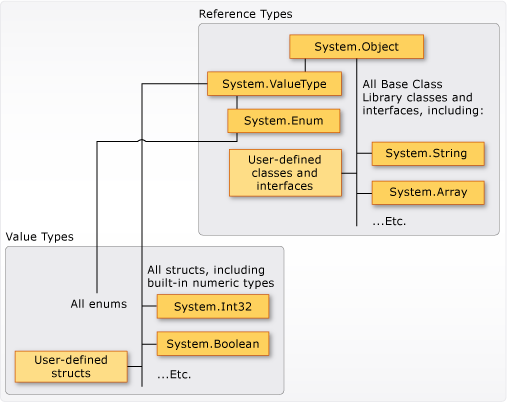
\includegraphics[width=140mm, height=100mm]{../img/value-reference-types-common-type-system.png}
\caption{The C\# type system \cite{online:cSharpTypeSystem}.}
\label{img04:typeSys}
\end{figure}
\par
\info{Nullability analysis}
C\# type inference infers, besides a type, its nullability, determining if it is possible to assign \texttt{null} value to that type.
C\# implicitly allows to assign \texttt{null} values to reference types indicating invalid value.
Since C\# 2.0 \cite{online:csHist}, it allows to assign \texttt{null} values to nullable value types, which are generic wrappers around value types.
Because assigning \texttt{null} value is referred to as a billion-dollar mistake, C\# 8.0 introduces optional settings prohibiting it and created nullable reference types explicitly allowing \texttt{null} assignment as a way of interaction with legacy code not using the feature.
\par
\info{Generic types and methods}
An essential part of the type system is C\# Generics, allowing parametrization of types and methods by other types. 
An example of a generic class is \texttt{System.Collections.Generic.List<T>} representing resizeable mutable array where  \texttt{T} represents arbitrary data type, which we want to have a collection of. 
Providing a type argument for  \texttt{T}, we create a new type where the type argument replaces the usages of  \texttt{T}.
\par
\info{Generic constraints}
Because a type parameter can be arbitrary, C\# treats it as a \texttt{System.Object}, which is insufficient in cases where the type parameter should provide special behaviour distinct from \texttt{System.Object}.
This requirement is achieved by type constraints, which restrict a set of types that can be passed to the parameter.
Several types of restrictions can be applied to type parameters in order to enable more actions on values of the restricted type parameters.
We can see examples of type constraints in the following code \ref{img05:typeConst}, where we use implementation restriction forcing the \texttt{T} to implement an interface providing API for comparing values with the same type.
The second restriction forces the type argument to have a default constructor.
Another restriction concerns an obligation that the type will be a value type or the type has to be non-nullable.
\par
\begin{figure}
\begin{lstlisting}
class MyList<T> : where T : IComparable<T>, new()
{  
	private T[] myBuffer;
	
	int CompareOnIndicies(int idx1, int idx2) {
		return myBuffer[idx1].CompareTo(myBufffer[idx2])	
	}
}
\end{lstlisting}
\caption{C\# type constraints.}
\label{img05:typeConst}
\end{figure}
\par
\info{Variance and contra-variance}
The last feature of generics influencing type inference is the concept of type variance.
Initially, type parameters are invariant, meaning an obligation to assign a generic type to another generic type having the same types of type parameters.
Generic interfaces introduce additional modifiers (\texttt{in}, and \texttt{out}) of type parameters, which allow to assign a type with the more specialized type argument to a type with the less specialized type argument or vice-versa respectively.
\par
\info{Overloading}
We end this subsection by presenting method overloading. 
C\# allows the definition of multiple methods with the same and count of type arguments having different parameters. 
We will see in the following chapters why this feature is one of the barriers to implement strong and efficient type inference.

\subsection{Relevant constructs}

\change{Dynamic}
\change{Implicit typed lambdas}
\change{Object creation expression and initializers}

%\par
%\info{Dynamic}
%C\# language is one of the languages contained in the .NET ecosystem.
%One of the goals of this ecosystem is to provide easy interaction with other .NET-compliant languages.
%Although \ac{CIL} of .NET is strongly typed, there are projects enabling a compilation of dynamically typed language to the \ac{CIL}.
%C\# \texttt{dynamic} keyword was introduced for interaction with these languages skipping type checking of values marked as \texttt{dynamic}.
%These values have a type of \texttt{object} and its method or type references are resolved during runtime.
%\par


%\subsection{Other constructs}

%\info{Implicitly typed lambdas}
%Anonymous functions also known as Lambdas are frequently used language features.
%Instead of declaring a dedicated method with a signature and a body, it allows to specify just the body with parameters on places, where a function delegate is required.
%\par
%\info{initializers}
%Initializers are used as a shortcut during an object instantiation.
%The most simple one is an object initializer that allows to assign values to the object's fields in a pleasant way instead of assigning them separately after the initialization.
%Array initializers are used to create fixed arrays with predefined content.
%Under the hood, each of the items in the initializer is assigned to the corresponding index of the array after the array creation.
%Collection initializers are similar to an array initializer defined on collections.
%Collections are types implementing \texttt{ICollection<T>} interface.
%One of the interface's declaring methods is \texttt{void Add<T>(T)} with adding semantic.
%Each type implementing this interface is allowed to use an initializer list in the same manner as an array initializer.
%It's just a sugar code hiding to call the `Add` method for each item in the initializer list.

\subsection{Type inference}

\change{Method type inference}
\change{Array type inference}
\change{Target-typed inference}



\section{Roslyn}

\change{Overview of compilation pipeline}
\change{Binder}
\change{OverloadResolution}
\change{MethodTypeInferrer}
\change{NullableWalker}
\change{Dynamic biding vs. runtime binding}

\section{Hindley-Millner type inference}

\change{Hindley-Millner type system}
\change{Set of rules}
\change{Restriction and possible extensions}

\section{Rust type inference}

\change{Rust type system}
\change{Type inference context}
\change{Type inference across multiple statement}
\change{Constructor type inference}

\section{Github issues}

\change{Mention related Github issues and csharplang repo.}
\change{Roslyn and csharplang repo}
\change{Proposal champions}
\change{Related issues}
